%% Cahpter_Zusammenfassung.tex
%%

%% ===========================
\chapter{Fazit und Ausblick}
\label{ch:Ergebnis}
%% ===========================

In diesem abschließenden Kapitel werden die Ergebnisse der Arbeit in ihren wichtigsten Punkten zusammengefasst und anhand der Anforderungen aus Kapitel \ref{ch:Systemanalyse:sec:Anforderungsanalyse} bewertet. Anschließend wird ein Ausblick auf weiterführende Möglichkeiten, sowie zukünftige Verbesserungsmöglichkeiten gegeben. 

%% ===========================
\section{Zusammenfassung}
\label{ch:Ergebnis:sec:zusammenfassung}
%% ===========================

In der vorliegenden Arbeit wurde ein System zur Bewertung von Beziehungen entwickelt. Hierzu wurden zuerst alle relevanten Komponenten von CAS genesisWorld untersucht. Dabei wurden Tabellen und Spalten identifiziert, die zur Umsetzung des neuen Systems notwendig sind. Anschließend wurden die Anforderungen an das neue System erhoben. Mit dem Wissen über die zu übernehmenden Daten und den Anforderungen wurden unterschiedliche  Datenbanksysteme hinsichtlich ihrer Eignung untersucht und sich für die H2-Datenbank entschieden. Die Entscheidung zugunsten der H2-Datenbank ist primär auf ihre Eigenschaften, die eine gute Performance versprechen, zurückzuführen.   

Aufbauend auf der zuvor ausgewählten Datenbank wurden Konzepte zur Umsetzung des Systems entwickelt. Bei der Konzeption wurde deduktiv vorgegangen. Zuerst wurde die Architektur definiert und anschließend die einzelnen Komponenten detailliert geplant. Bei der Planung wurde nicht versucht ein universell einsetzbares System zu entwickeln, sondern vielmehr eine domänenspezifische Lösung für das Szenario auszuarbeiten. Nachdem alle Technologien sowie Vorgehensweisen festgelegt wurden, ging man auf die Umsetzungen ein. In der Umsetzung wurden die konkreten Funktionsweisen und Implementierungen der einzelnen Komponenten vorgestellt. Schlussendlich wurden die fertige Oberfläche und die getroffenen Designentscheidungen aufgezeigt.
 
%% ===========================
\section{Bewertung der Ergebnisse}
\label{ch:Ergebnis:sec:bewertung}
%% ===========================

Die funktionalen Anforderungen konnten alle umgesetzt werden und wurden bereits im vorherigen Kapitel erläutert. Im Folgenden wird somit auf die Erfüllung der nicht funktionalen Anforderungen eingegangen. Zu ihnen zählt die Möglichkeit das System nur auf einem Rechner zu betreiben, kurze Antwortzeiten des Systems, lose Kopplung zwischen den Webprojekten und ein gewisses Maß an Portabilität zu erreichen. Die Bewertung des Ergebnisses erfolgt anhand der Gegenüberstellung von Anforderungen und den Charakteristika des Systems.

Die erste Anforderung konnte durch den Einsatz eines einzigen Servers eingehalten werden. Weiterhin wurde eine lose Kopplung zwischen Server und Client erreicht. Diese spiegelt sich in den REST-Schnittstellen der jeweiligen Komponenten wieder. Überdies gibt es keine Abhängigkeiten zwischen den Klassen der Darstellung und den Klassen der Geschäftslogik. Ein gewisses Maß an Portabilität wurde vorausgesetzt, damit ein Verlagern des Systems auf andere Instanzen kein Problem darstellt. Dies wurde durch die Verwendung der Web-Archive-Dateien erreicht. Sie ermöglichen den Einsatz auf verschiedenen Tomcat Servern, was sie nicht nur portabel, sondern auch auf verschiedenen Servern einsetzbar macht. 

Die wichtigste Anforderung ist eine kurze Antwortzeit des Systems. Tabelle \ref{tb:vergleichAbfragegeschwindigkeit} zeigt, dass dieser Forderung nachgekommen wird. Ebenfalls deutlich zu erkennen ist die Auswirkung des geänderten Schemas. Der Sprung von 98.000ms auf 350ms ist durch die Reduktion in der Abfragekomplexität zu erklären. Die Abfragen erfolgen über wesentlich weniger Tabellen und Spalten als zuvor. Außerdem wird im neuen Schema kein Verbund in der Datenbankabfrage mehr benötigt. Allerdings ergeben sich durch derartigen Maßnahmen, wie sie im Schemadesign ergriffen wurden, Probleme bei zukünftigen Erweiterungen. Ein Grund dafür ist die  geringe Normalisierung innerhalb des Schemas. Beispielsweise könnte  entschieden werden den Ort eines Termins in die Tabelle \textit{Data} aufzunehmen. Dadurch würden lediglich in den Tupeln die Ortsbezeichnungen stehen. In allen anderen Tupeln würde die Spalte Nullwerte enthalten. Werden noch weitere Attribute hingezogen resultieren daraus sehr viele leere Felder in der Datenbank, wodurch unnötig Speicherplatz verbraucht wird. Gerade durch die Datenhaltung im Hauptspeicher stellen derartige Umstände ein Problem dar. Um dem entgegenzuwirken müsste die Datenbank weiter normalisiert werden. Bei der Normalisierung würde es allerdings auch zu gewissen Performance-Verlusten kommen.

\begin{table}[htbp]
\centering
\begin{tabular} {l | r}
Versuchskomponente & Zeit in ms  \\ \hline
MSSQL Datenbank \& Altes Schema & 98000 \\
MSSQL Datenbank \& Neues Schema & 750 \\
H2 Datenbank \& Neues Schema & 80 \\
\end{tabular}
\caption{Abfragegeschwindigkeit Vergleich}
\label{tb:vergleichAbfragegeschwindigkeit}
\end{table}

Es stellt sich weiterhin die Frage ist die Datenbank nur aufgrund des neuen Schemas schneller? Um dieser Frage nachzugehen wurden Tests durchgeführt. Abbildung \ref{ergebniss_vergleich} zeigt die Ergebnisse dieser Testreihen. Alle Testläufe wurden mit einem Rechner durchgeführt. Dieser simulierte mithilfe von Multithreading den gleichzeitigen Zugriff von 100 Benutzern. Die in den Diagrammen angegebene Zeit bezieht sich somit auf die Ausführung aller 100 Abfragen. Jeder simulierte Benutzer führt die auf der y-Achse angegebene Anzahl an Abfragen aus. Beim obersten Balken in (a) sind es beispielsweise 15 Mio. SELECT-Anweisungen pro Benutzer. In (b) hingegen wird die Verarbeitungsgeschwindigkeit bei Updates verglichen. Ein Vergleich der Performance bei Insert-Anweisungen ist in (c) dargestellt.    

\begin{figure}[htbp]
\centering
\subfigure[Vergleich anhand Select-Operationen]{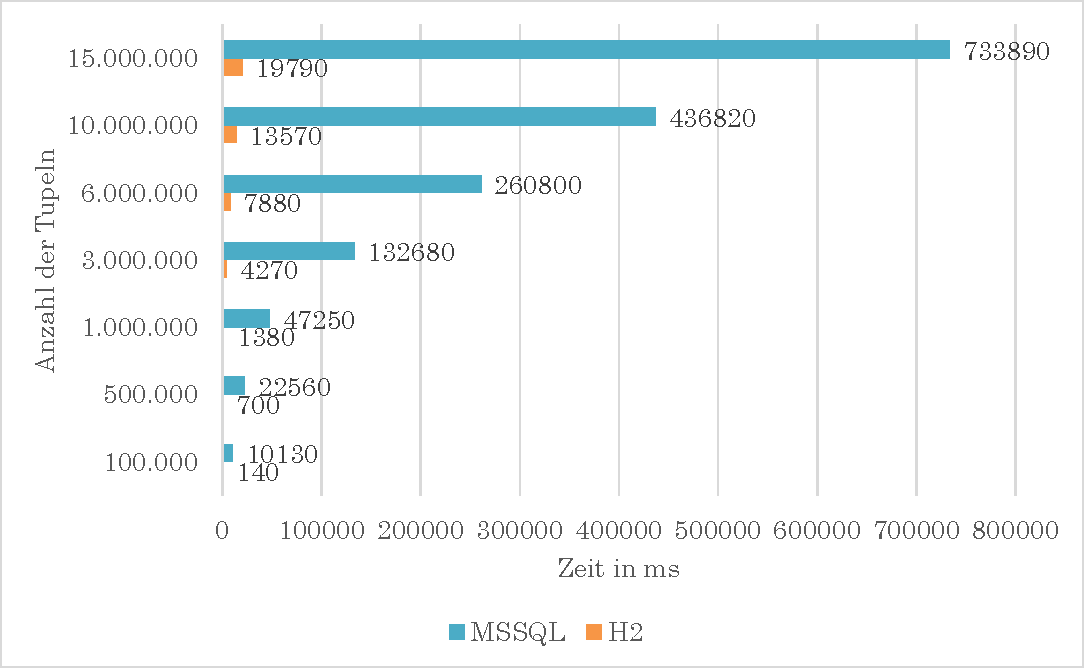
\includegraphics[width=0.49\textwidth]{charts/select.pdf}}\hfill
\subfigure[Vergleich anhand Update-Operationen]{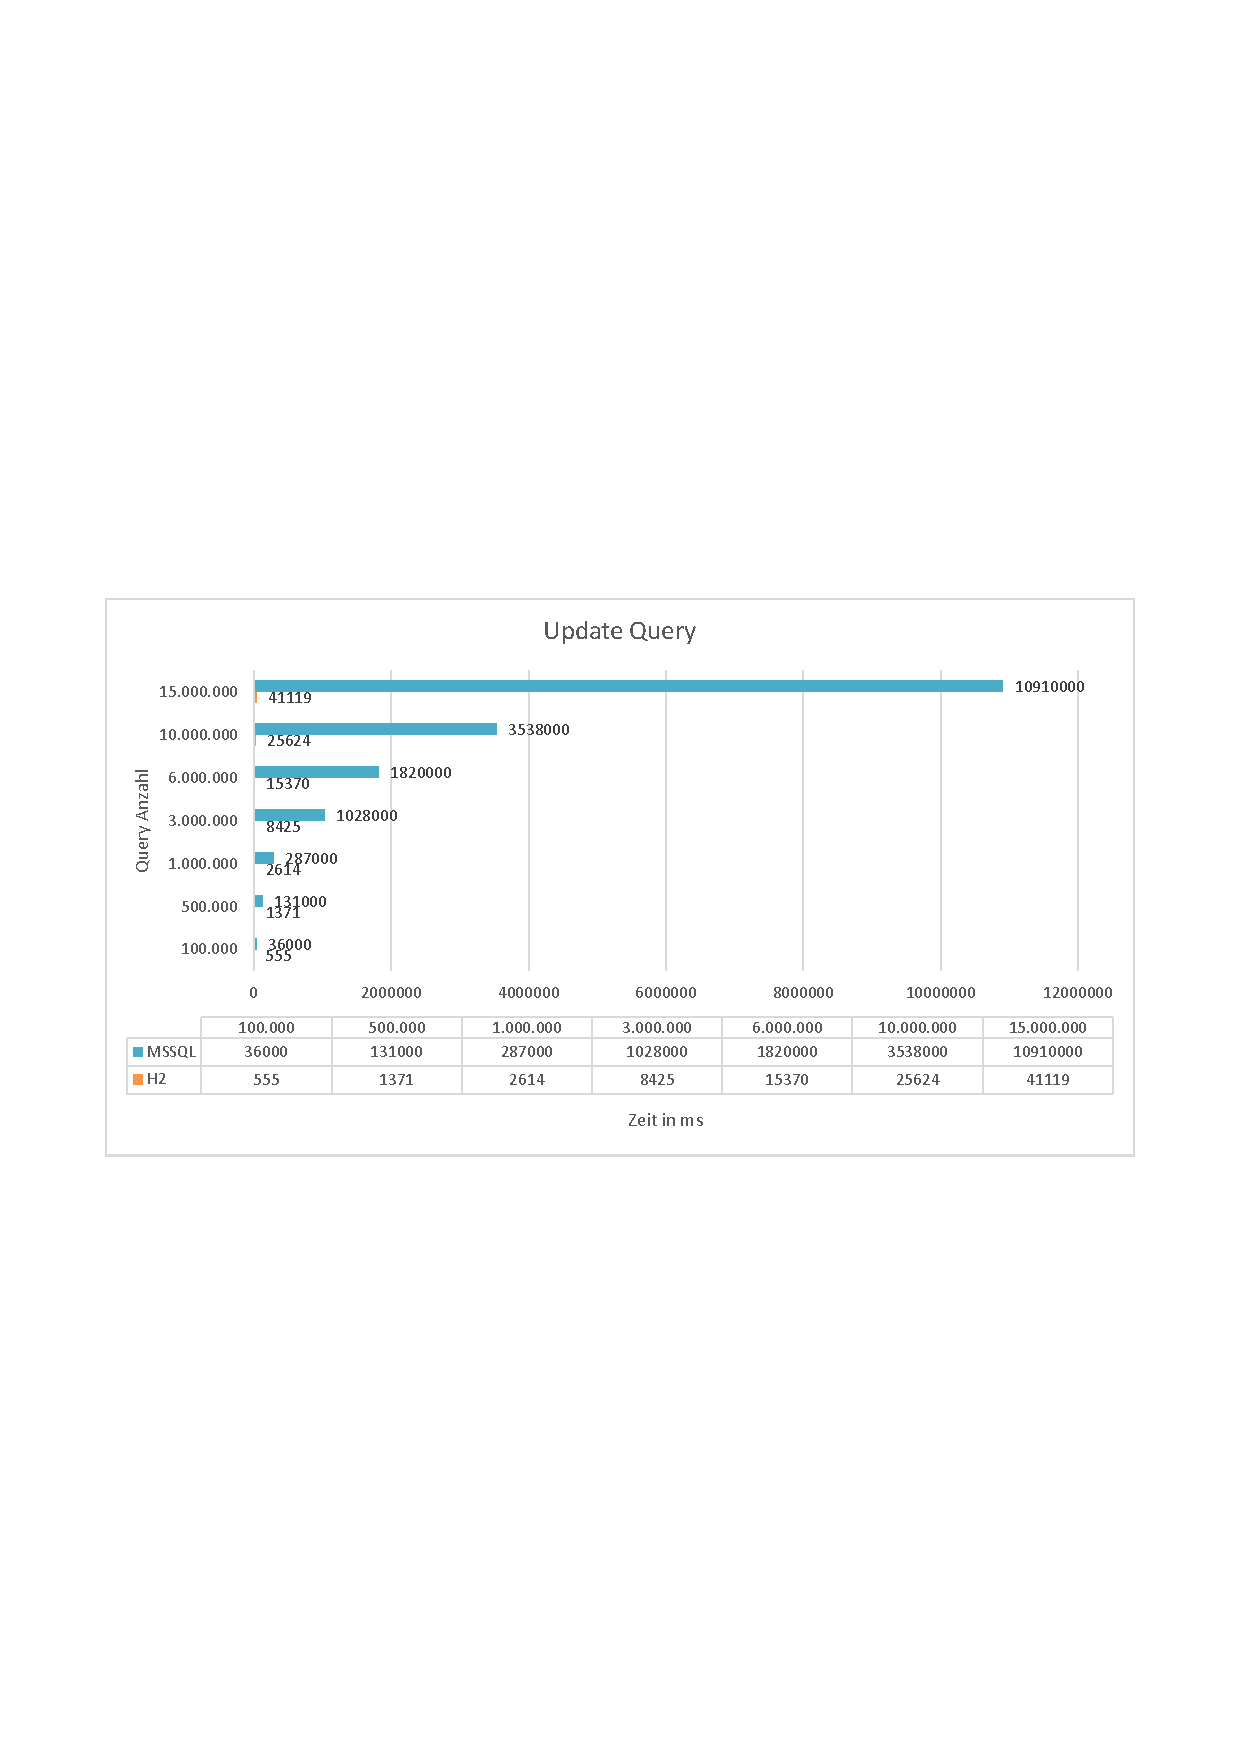
\includegraphics[width=0.49\textwidth]{charts/update.pdf}}\hfill
\subfigure[Vergleich anhand Insert-Operationen]{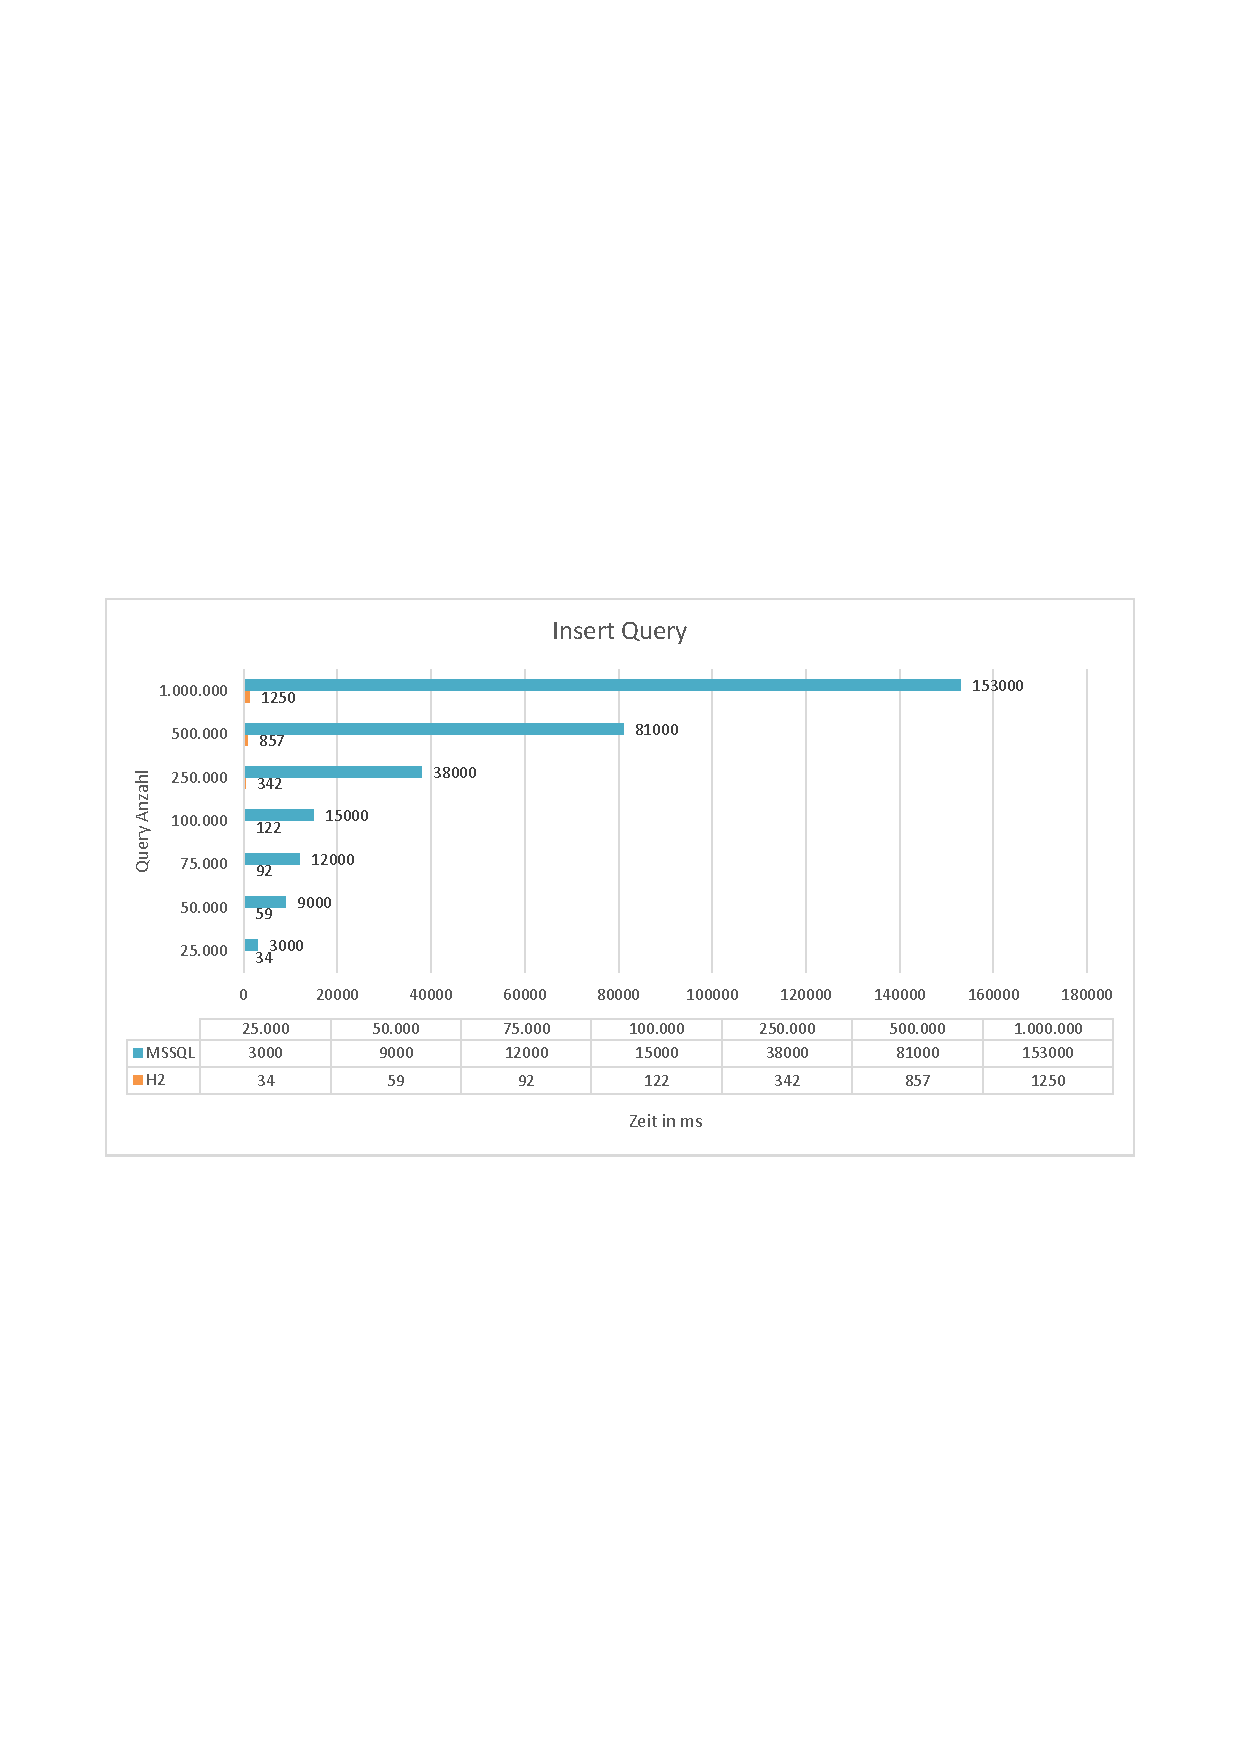
\includegraphics[width=0.5\textwidth]{charts/insert.pdf}}
\caption{Vergleich von Antwortzeiten}
\label{ergebniss_vergleich}
\end{figure}

Die Ergebnisse der Tests zeigen, dass die H2-Datenbank bei den durchgeführten Tests deutlich schneller als die MSSQL Datenbank ist. Die H2-Datenbank ist bei SELECT-Anweisungen um den Faktor 37 schneller. Bei Update-Anweisungen sogar um den Faktor 117. Ebenso bei Insert-Anweisungen, die einen Unterschied um den Faktor 124 aufweisen. Daraus lässt sich ableiten, dass die H2-Datenbank durch ihre In-Memory-Tabellen deutlich an Performance gewinnt. Diese wird zum Teil durch den Verzicht auf Persistenz erlangt. Würde die Datenbank ihre Daten zur Sicherung auf die Festplatte schreiben, müsste bei Schreiboperationen mit Verschlechterungen in der Performance gerechnet werden. Im vorliegenden System, welches fast nur Leseoperationen durchführt, stellen die nicht persistenten Tabellen allerdings kein großes Defizit dar. Ausschlaggebend für die Schnelligkeit ist allerdings die Nutzung des Hauptspeichers als Speichermedium. Dessen Gebrauch könnte allerdings in der Zukunft aufgrund der immer größer werdenden Datenmengen ein Problem darstellen.  

%% ===========================
\section{Ausblick}
\label{ch:Ergebnis:sec:Ausblick}
%% ===========================

Mit der Umsetzung des in der Arbeit beschriebenen Systems steht eine performante Lösung bereit, die eine Bewertung von Beziehungen zwischen Personen aus einer CRM-Lösung ermöglicht.

Die Bewertung der Beziehungen beruht derzeit lediglich auf der Anzahl von CRM-Objekten, die zwischen Personen geteilt werden. Dementsprechend wird nur die Häufigkeit gewertet. Um die Bewertung einer Beziehung genauer feststellen zu können, werden zusätzliche Regeln benötigt. Diese Regeln sollten auf psychologischen Erkenntnissen und Erfahrungswerten aufbauen. Durch Regeln ließe sich die Aussagekraft von Ergebnissen weiter steigern. Beispielsweise sind kommunikative Kontakte wie Telefonate oder E-Mail Verkehr, kein Indikator für Vertrauen. Die Einsicht in vertrauliche Dokumente setzt dagegen eine engere Zusammenarbeit bzw. Vertrauen voraus. Dies sollte somit stärker gewichtet werden. Um die zuvor genannten Funktionen umzusetzen muss das Schema allerdings erweitert und der ETL-Prozess angepasst werden, da diese Informationen derzeit nicht in der Datenbank vorhanden sind.

Mit dem System könnten zukünftig auch neue Erkenntnisse gewonnen werden. Beispielsweise können die Ergebnisse von erfolgreichen Mitarbeitern, mit den von weniger erfolgreichen Mitarbeitern verglichen werden. Mithilfe der Unterschiede könnten Rückschlüsse auf eventuelle Ursachen gezogen werden.

Weiterhin könnten die Vertriebsmitarbeiter mithilfe des Systems individuell unterstützt werden. Dazu müssten zusätzliche Informationen, die etwas über den Wert eines Kunden aussagen, ermittelt werden. Der Wert eines Kunden könnte sich zum Beispiel aus den durch ihn gewonnen Einnahmen ergeben. Unter den Kunden müsste wie bei den Beziehungen ein Ranking der Ergebnisse aufgestellt werden. Nun könnten die beiden Rankings auf Diskrepanzen verglichen werden. Dadurch ist ein Vergleich zwischen dem Wert eines Kunden und der Beziehung mit ihm möglich. Auf diese Weise könnten zu große Unterschiede im betriebenen Aufwand und dem Nutzen des Kunden entdeckt werden. 

Eine weitere Möglichkeit ist die Reihenfolge der Ergebnisse umzukehren. Dadurch könnten Kundenbeziehungen auf mangelhafte Kundenpflege hin untersucht werden. Dazu müsste lediglich eine Anpassung an der SQL-Abfrage vorgenommen werden.

Überdies könnten Ergebnisse verschiedener Personen verglichen werden. Der Vergleich könnte dabei unter Personen aus einer Gruppe oder aus selbst erstellten Personenkonstellationen erfolgen. Auf Vertriebsmitarbeiter angewandt könnte überprüft werden, ob die Verteilung der Kunden auf einzelne Mitarbeiter effizient gestaltet ist. Beispielsweise läse sich damit feststellen, ob zu viele Mitarbeiter sich unwissentlich auf denselben Kunden konzentrieren.

Eine andere weiterführende Möglichkeit bietet sich in der Bewertung einer Beziehung  über verschiedene Zeitpunkte hinweg. Dadurch könnten zeitliche Entwicklungen im Kontakt der Mitarbeiter mit dem Kunden erkannt werden. Liniendiagramme wären dabei eine geeignete Form der Visualisierung, da sich mit ihnen zeitliche Abläufe gut darstellen lassen. Der Datenbestand bietet die Möglichkeiten dies umzusetzen, allerdings müssen entsprechende Abfragen und Darstellungen implementiert werden.  
